\newcommand{\plotsize}{0.45\textwidth}

%%%%%%%%%%%%%%%%%%%%%%%%%%%%%%%%%%%%%%%%%%%%%%%%%%%%%%%%%%%%%%%%%%%%%%

\section{Experimental Results}
\label{results}

This section presents initial results for our VM. First, we present a
comparison with similar programs written in other programming
languages in order to show evidence that our VM is viable. Then, we
present scalability results in order to show that LM programs can take
advantage of multicore architectures.

For our experimental setup, we used a machine with 32 (2x16) Core AMD
Opteron (tm) Processor 6274 $@$ 2.2 GHz with 32 GBytes of RAM memory
and running the Linux kernel 3.8.3-1.fc17.x86\_64.  We compiled our VM
using GCC 4.7.2 (g++) with the flags \texttt{-O3 -std=c+0x
  -march=x86-64}. We run all experiments 3 times and averaged the
execution time.

%%%%%%%%%%%%%%%%%%%%%%%%%%%%%%%%%%%%%%%%%%%%%%%%%%%%%%%%%%%%%%%%%%%%%%

\subsection{Absolute Execution Time}

To put our VM in perspective, we first compare it in terms of absolute
execution time with other competing systems using a single thread.

In Table~\ref{tbl:comp_nqueens}, we compare LM's version of the
classic N-Queens puzzle against 3 other versions: a straightforward
sequential program implemented in C using backtracking; a sequential
Python implementation~\cite{vanRossum:1995:PRM}; and a Prolog
implementation executed in YAP
Prolog~\cite{DBLP:journals/corr/abs-1102-3896}, an efficient
implementation of Prolog. Numbers less than 1 mean that LM is faster
and larger than 1 mean that LM is slower. We can observe that LM
easily beats Python, but is 5 to 10 times slower than YAP Prolog and
around 15 times slower than C. Note however that, as we will see next,
if we use at least 16 threads in LM, we can beat the sequential
implementation written in C.

\begin{table}[ht]
\centering
{\begin{tabular}{c|c|c|c}
\textbf{Problem} & \multicolumn{3}{c}{\textbf{System}} \\
\textbf{Size} & \textbf{C} & \textbf{Python} & \textbf{YAP Prolog} \\
\hline\hline
\textbf{10x10} & 16.92 & 0.62 & 5.42 \\
\textbf{11x11} & 21.59 & 0.64 & 6.47 \\
\textbf{12x12} & 10.32 & 0.73 & 7.61 \\
\textbf{13x13} & 14.35 & 0.88 & 10.38 \\
\end{tabular}}
\caption{Comparing the absolute execution times (LM/System) for the
  N-Queens program}
\label{tbl:comp_nqueens}
\end{table}

In Table~\ref{tbl:comp_bp}, we compare LM's Belief Propagation (BP)
program, a machine learning algorithm to denoise images, against a
sequential C, Python and GraphLab~\cite{GraphLab2010} version of the
algorithm. GraphLab is a parallel C++ library used to solve
graph-based problems in machine learning. C and GraphLab perform about
the same since both use C/C++. Python runs very slowly since it is a
dynamic programming language and BP has many mathematical
computations. We should note, however, that LM's version uses some
external functions written in C++ in order to improve execution time,
therefore the comparison is not totally fair.

\begin{table}[ht]
\centering
{\begin{tabular}{c|c|c|c}
\textbf{Problem} & \multicolumn{3}{c}{\textbf{System}} \\
\textbf{Size} & \textbf{C} & \textbf{Python} & \textbf{GraphLab} \\
\hline\hline
\textbf{10}  & 0.67 & 0.03 & 1.00 \\
\textbf{50}  & 1.77 & 0.04 & 1.73 \\
\textbf{200} & 1.99 & 0.05 & 1.79 \\
\textbf{400} & 2.00 & 0.04 & 1.80 \\
\end{tabular}}
\caption{Comparing the absolute execution times (LM/System) for the
  Belief Propagation program}
\label{tbl:comp_bp}
\end{table}

We also compared a LM's version of the PageRank program against a
similar GraphLab version and LM showed to be around 4 to 6 times
slower. Our worse results were obtained for the all-pairs shortest
distance algorithm where a LM's version of the problem was around 50
times slower than a C sequential implementation of the Dijkstra
algorithm, but almost twice as fast when compared to the same
implementation in Python.

%%%%%%%%%%%%%%%%%%%%%%%%%%%%%%%%%%%%%%%%%%%%%%%%%%%%%%%%%%%%%%%%%%%%%%

\subsection{Scalability}

\begin{figure*}[ht]
\centering
\subfigure[PageRank using a graph of web pages with around 12,000 nodes and 292,000 edges]
   {\label{exp:pagerank}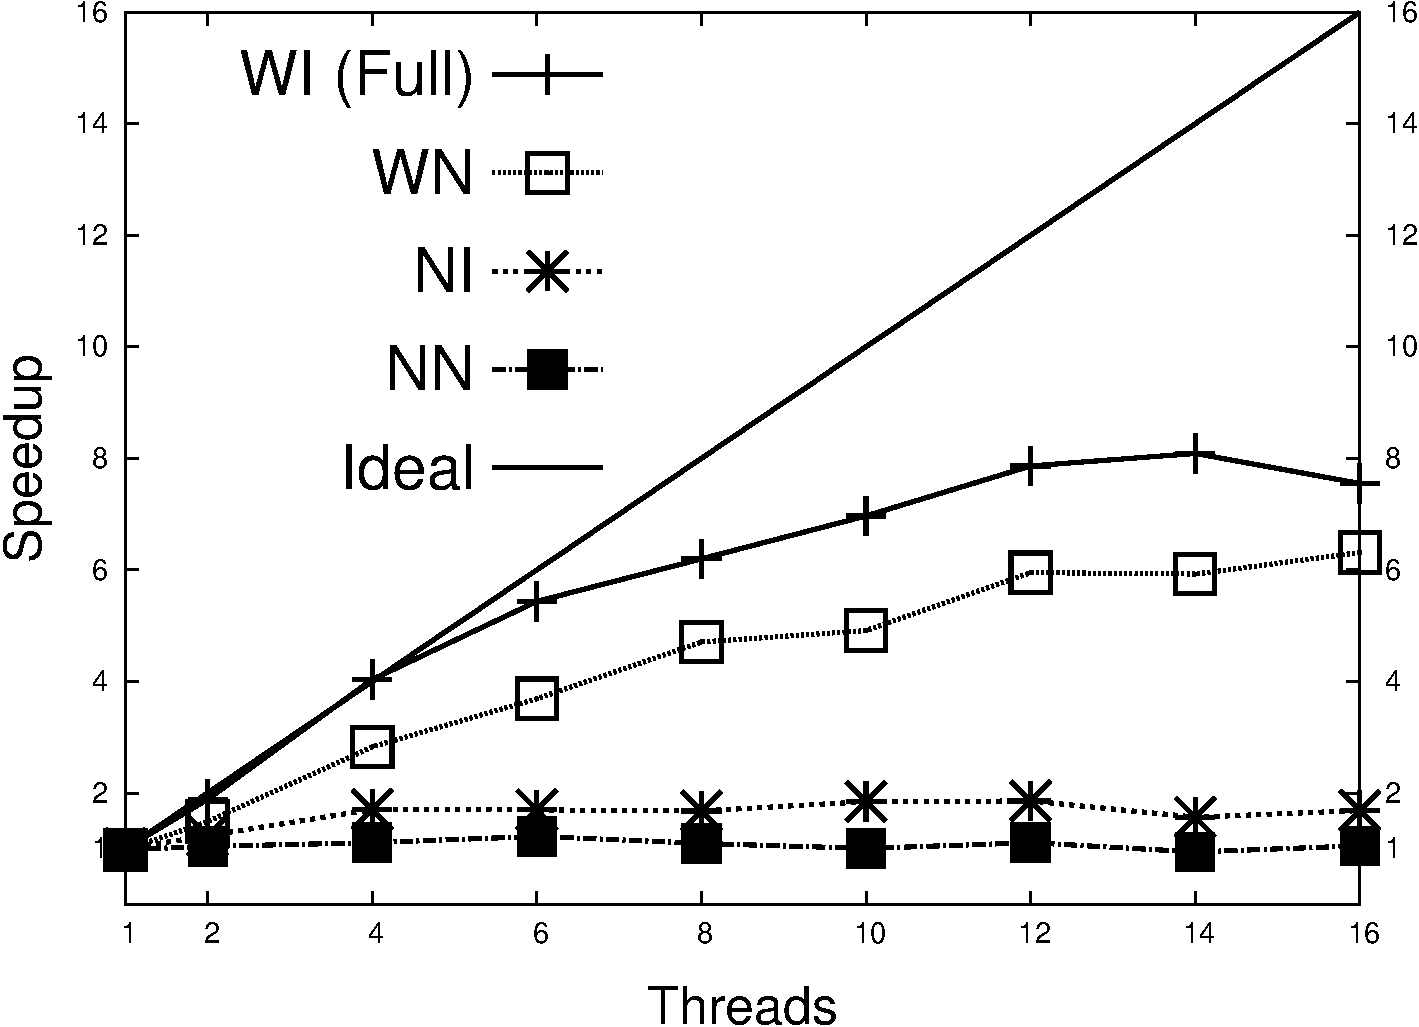
\includegraphics[width=\plotsize]{figures/results-pagerank-search-engines.pdf}}
\hspace{0.5cm}
\subfigure[GGC using a random graph with 2,000 nodes and 600,000 edges]
   {\label{exp:ggc}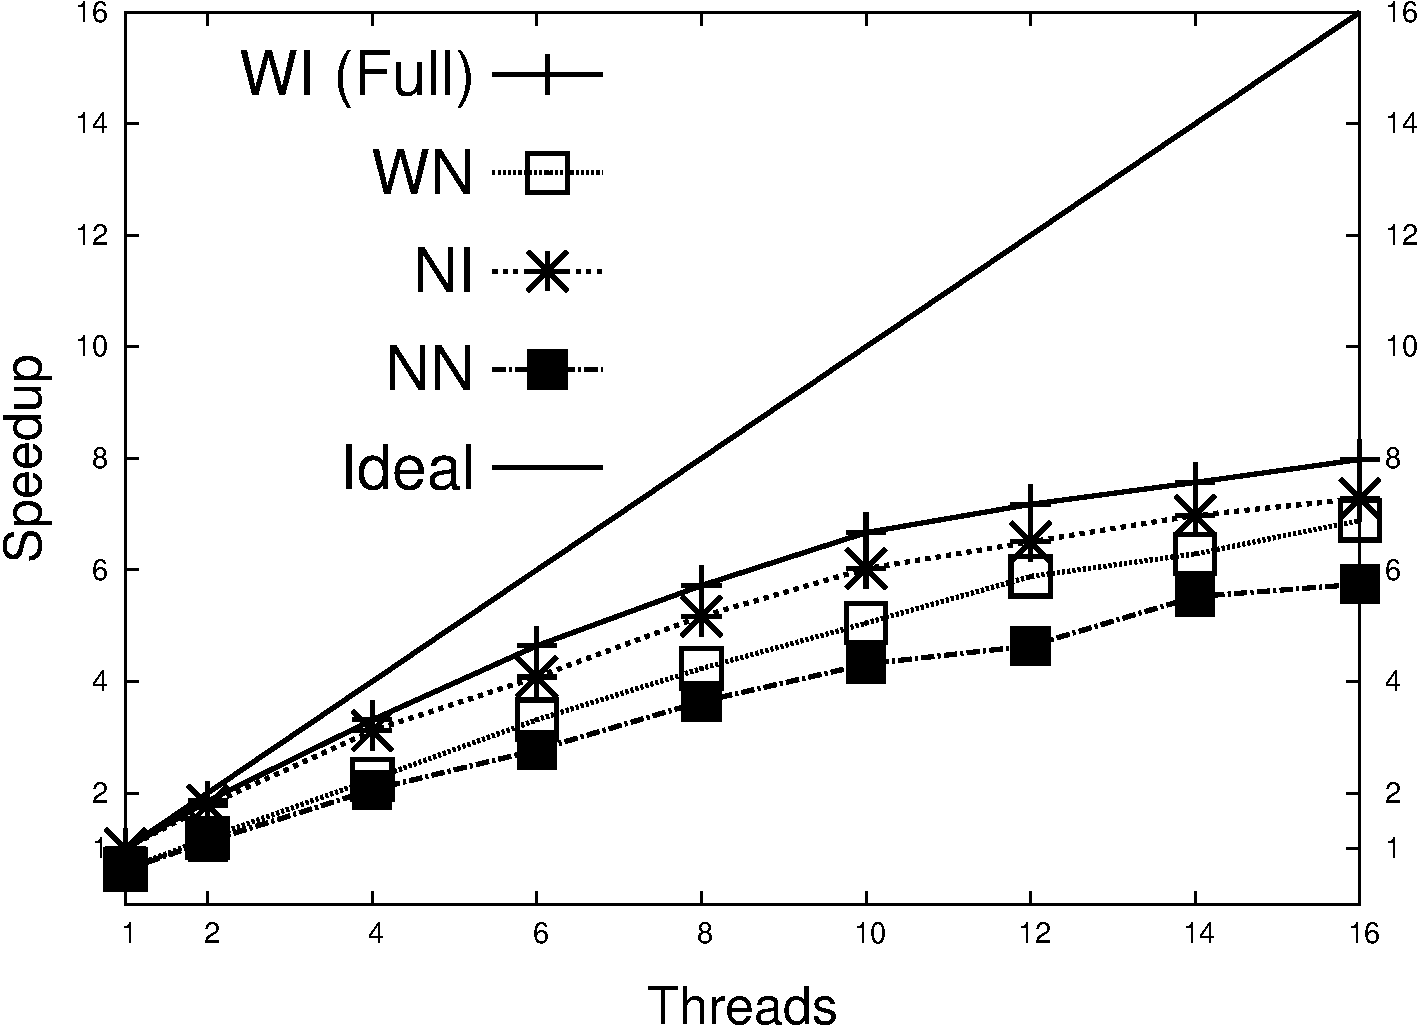
\includegraphics[width=\plotsize]{figures/results-ggc.pdf}}
\caption{Experimental results for the GGC and PageRank algorithms}
\end{figure*}

\begin{figure*}[ht]
\centering
\subfigure[Shortest Distance for a graph with around 5,000 nodes and 13,000 edges]
   {\label{exp:sd}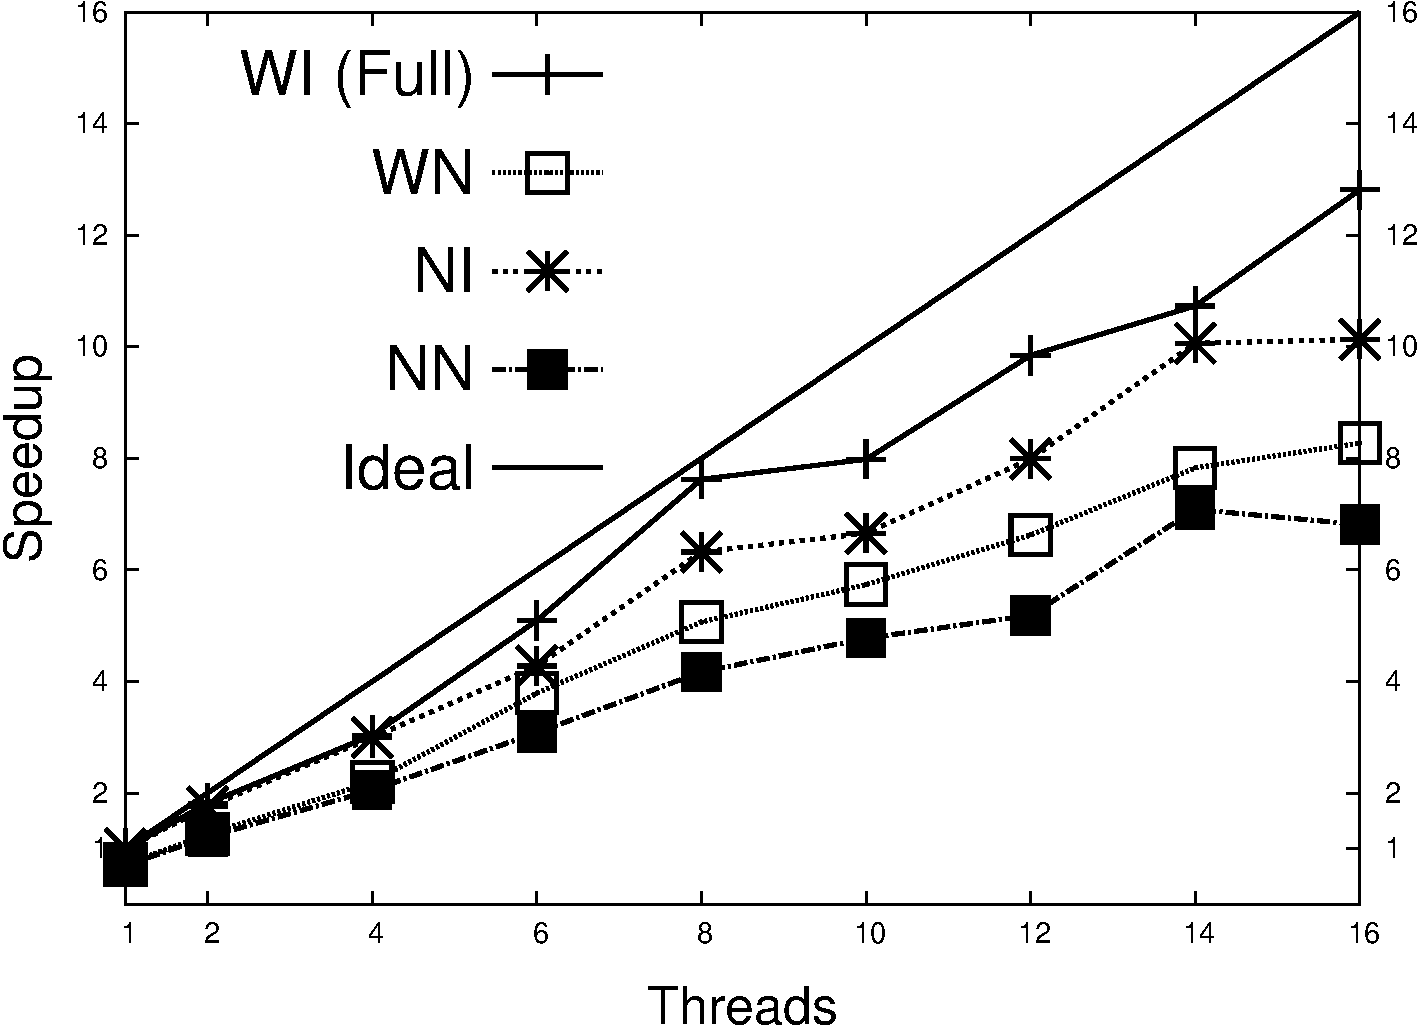
\includegraphics[width=\plotsize]{figures/results-shortest-uspowergrid.pdf}}
\hspace{0.5cm}
\subfigure[MiniMax algorithm for the Tic-Tac-Toe game (complete tree)]
   {\label{exp:minimax}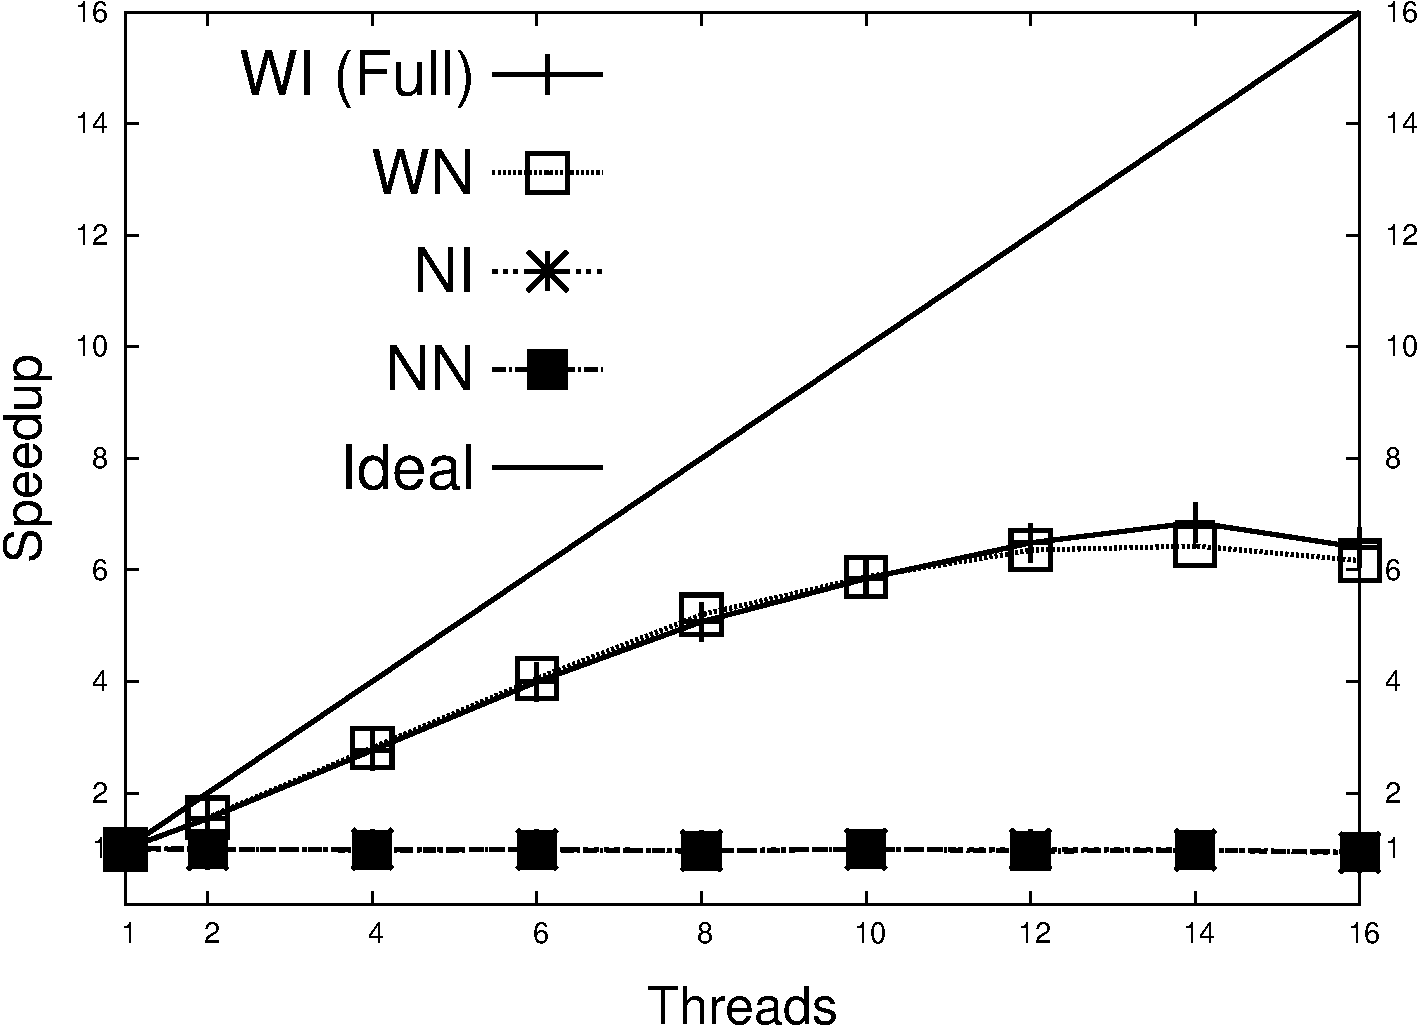
\includegraphics[width=\plotsize]{figures/results-minimax.pdf}}
\caption{Experimental results for the Shortest Distance and MiniMax algorithm}
\end{figure*}

\begin{figure*}[ht]
\centering
\subfigure[N-Queens program (13x13~board)]
   {\label{exp:13queens}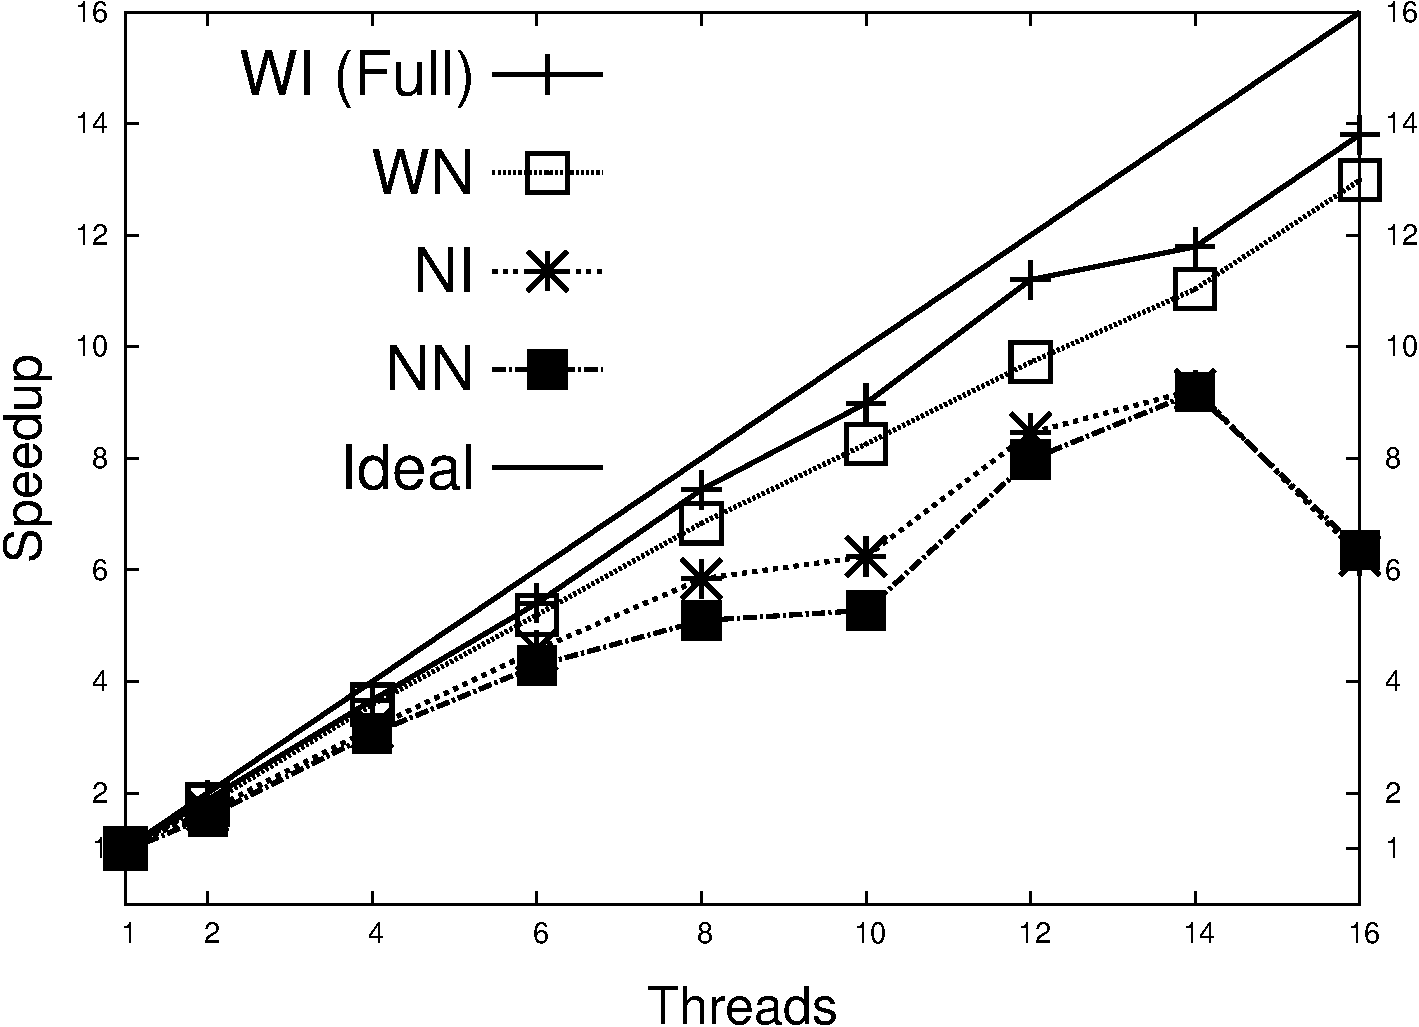
\includegraphics[width=\plotsize]{figures/results-13queens.pdf}}
\hspace{0.5cm}
\subfigure[BP (400x400~image)]
   {\label{exp:bp}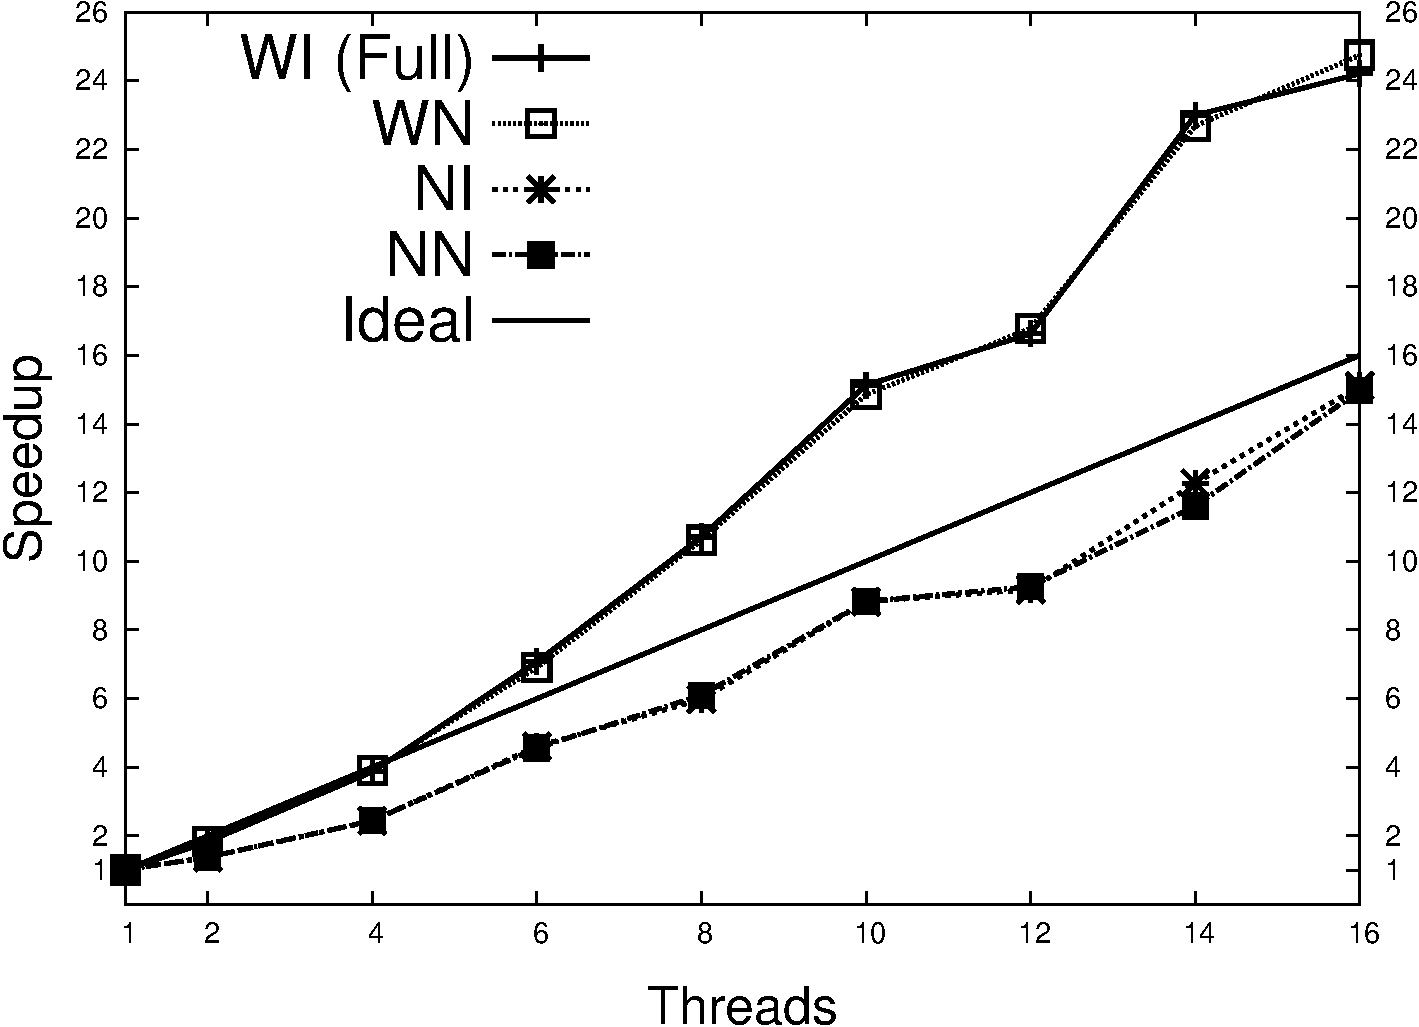
\includegraphics[width=\plotsize]{figures/results-bp.pdf}}
\caption{Experimental results for the N-Queens and Belief Propagation programs}
\end{figure*}

In this section we measure the scalability of the VM along with the
performance gains due to work stealing and dynamic indexing.  For
this purpose, we used 4 configurations for the VM: \textbf{WI}, the
full configuration that includes work stealing and dynamic indexing;
\textbf{WN}, with work stealing but without dynamic
indexing; \textbf{NI}, with indexing but without work stealing; and
\textbf{NN}, without work stealing and without dynamic indexing.  We
ran each configuration using 1, 2, 4, 6, 8, 10, 12, 14 and 16 threads
and compared the run time against the sequential execution (1 thread)
of \textbf{WI}. We used the following set of programs:

\begin{itemize}
\item PageRank implements a PageRank algorithm without synchronization
  between iterations. Every time a node sends a new rank to its
  neighbors and the change was significant, the neighbors are
  scheduled to recompute their ranks.
\item Greedy Graph Coloring (GGC) colors nodes in a graph so that no
  two adjacent nodes have the same color. We start with a small number
  of colors and then we expand the number of colors when we cannot
  color the graph.
\item Shortest Distance (SD) computes the shortest distance of all
  nodes to all nodes.
\item MiniMax, the AI algorithm for selecting the best player move in a game of Tic-Tac-Toe.
\item N-Queens, the classic puzzle for a 13x13 board.
\item Belief Propagation, a machine learning algorithm to denoise
  images.
\end{itemize}

The PageRank results are shown in Fig.~\ref{exp:pagerank}. We used a
search engine graph of 12,000 webpages\footnote{Available from
  \url{http://www.cs.toronto.edu/~tsap/experiments/download/download.html}}. Since
this dataset follows the power law, that is, there is a small number
of pages with a lots of links (1\% of the nodes have 75\% of the
edges), it can be difficult to parallelize. Our results show that the
VM is able to scale the program with up to 14 threads.  We also notice
the huge performance drop when we run the VM without work
stealing. Dynamic indexing is also an advantage, since it detects that
the facts for the pagerank of neighboring nodes need to be indexed
efficiently.

Figure~\ref{exp:ggc} presents the results for the GGC program with a
random dataset of 2,000 nodes with an uniform distribution of edges.
There is a slight drop in scalability as the number of threads goes
up, but the VM is still capable of reducing the run time. We note that
in this program, the work available is reduced as the graph becomes
increasingly colored.

In Fig.~\ref{exp:sd} we show the results for the Shortest Distance program.
We attain a 13-fold speedup for 16 threads with both work stealing and dynamic
indexing (\textbf{WI}). We note that indexing is more advantageous than work stealing
because indexing the distance facts according to the source node is more crucial
than improved load balancing.

The results for the MiniMax algorithm are presented in Fig.~\ref{exp:minimax}.
MiniMax is very different than the other algorithms because the graph of nodes is dynamic
and is created during program execution. The load balancing is also problematic since there
is little work to do in the initial and final phases of the algorithm. Still, our VM has decent
performance, with almost a 7-fold speedup for 14 threads. The scalability drops with 16 threads
but we think that is due to the simplicity of the current work stealing algorithm.
Dynamic indexing has no effects in this program.

The results for the N-Queens program are shown in
Fig.~\ref{exp:13queens}. The program is not regular since computation
starts at the top of the grid and then rolls down, until only the last
row be doing computation. Because the number of valid states for the
nodes in the upper rows is much less than the nodes in the lower rows,
this may potentially lead to load balancing problems. The results show
that our system is able to scale well. When work stealing is left out
(\textbf{NI} and \textbf{NN}), we see a serious drop in performance with 16 threads.

Finally, we shown the results for the Belief Propagation~(BP) program
in Fig.~\ref{exp:bp}. BP is a regular and asynchronous program and
benefits (as expected) from having multiple threads executing since
the belief values of each node will converge faster.  The super-linear
results prove this assertion.

\subsection{Memory Statistics}

In this section, we present the amount of \textbf{Memory} used by the VM after the
programs presented in the previous section complete. We also count the number of
\textbf{Facts} stored in the database. This serves as an indication of
how much memory is needed in terms of the number of facts stored in the database.
Results are shown in Table~\ref{tbl:memory}.

\begin{table}[ht]
\centering
{\begin{tabular}{c|c|c|c}
\textbf{Program} & \textbf{Facts} & \textbf{Memory} & \textbf{Per Fact} \\
\hline\hline
PageRank & 1,180,603 & 203,832 KB & 176 bytes \\
GGC & 2,363,536 & 292,682 KB & 127 bytes \\
SD & 502,347 & 45,387 KB & 92 bytes \\
MiniMax & 3 & 886,443 KB & 295,481 KB \\
N-Queens & 74,557 & 55,408 KB & 760 bytes \\
BP & 2,235,200 & 617,417 KB & 283 bytes \\
\hline\hline
\multicolumn{3}{l}{Average (W/ MiniMax) } & 288 bytes \\
\end{tabular}}
\caption{Memory usage of programs after completion using 1 thread.}
\label{tbl:memory}
\end{table}

The most unexpected result in Table~\ref{tbl:memory} is that of the MiniMax program. There is a
very low number of facts (that indicate the final player decision) and a huge
amount of memory. How can this be explained? We note that MiniMax builds a huge
decision tree of nodes with almost $9!$ leaves. Although these nodes do not participate
in the computation after the MiniMax result is computed for them, the VM does not garbage collect
nodes that do not contain facts and that do not have external references from other nodes.
This is a potential improvement that can be done in the future.

PageRank, GGC and SD show a low memory usage per fact. This makes sense since the predicates
used in those programs are relatively simple with only a few arguments.
This changes with the N-Queens problem where the predicates have lists representing the valid
positions of the queens in the board. Storing lists is far more expensive than storing integral
values such as integers or floating point numbers. The same thing happens with BP because
the belief values are stored as lists of floating point numbers.